\chapter{EM vlny v anizotropním prostředí}
\section{Vlnová rovnice v anizotropním prostředí}
Vlnová rovnice pro světlo v anizotropním, tedy homogením nevodivém bez nábojů a proudů, prostředí se dá snadno odvodit z Maxwellových rovnic
\begin{eqnarray}
\nabla \times\vec{H} - \frac{\partial\vec{D}}{\partial t} &=& 0 , \label{Max1} \\
\nabla \cdot \vec{D} &=& 0, \label{Max2} \\
\nabla \times \vec{E} + \frac{\partial \vec{B}}{\partial t} &=& 0, \label{Max3}\\
\nabla\cdot\vec{B}&=&0 \label{Max4}
\end{eqnarray}
Na optických frekvencích můžeme počítat, že $\mu_r\approx1$ a tedy platí $\mu=\mu_0$. Prostředí je tedy charakterizováno tenzorem permitivity $\varepsilon$. Tento tenzor má obecně tvar
\begin{eqnarray}
\varepsilon=
\begin{bmatrix}
\varepsilon_{xx} & \varepsilon_{xy} & \varepsilon_{xz} \\
\varepsilon_{yx}& \varepsilon_{yy}& \varepsilon_{yz} \\
\varepsilon_{zx}& \varepsilon_{zy}& \varepsilon_{zz}
\end{bmatrix}
\end{eqnarray}
Dále vhodné zavést tzv. redukovaný vlnový vektor, který zančíme $\vec{N}$ a je definován
\begin{eqnarray}
\vec{N}=\frac{c}{\omega}\vec{k} = (N_x\vec{i_x}+N_y\vec{i_y}+N_z\vec{i_z})
\end{eqnarray}
Standartní řešení ve tvaru rovinné vlny
\begin{eqnarray}
\vec{E} &=& \vec{E_0}e^{[-i(\omega t-\vec{k}\cdot\vec{r})]}, \\
\vec{B} &=& \vec{B_0}e^{[-i(\omega t-\vec{k}\cdot\vec{r})]}
\end{eqnarray}
dává po dosazení do rovnic (\ref{Max1}) a (\ref{Max2})
\begin{eqnarray}
\vec{k}\times(\vec{k}\times\vec{E}) + \frac{\omega^2}{c^2}\varepsilon\vec{E}=0
\end{eqnarray}
Tuto vektorovou rovnici můžeme rozepsat pro složky vektorů za pomoci Levi-Civitova symbolu $\epsilon$ do tvaru
\begin{eqnarray}
\epsilon_{ijk}k_j\epsilon_{klm}k_lE_m+\frac{\omega^2}{c^2}\varepsilon_{ij}E_j =0
\end{eqnarray}
Postupnou úpravou, která je podrobněji popsána v \cite{Nyvlt} a volbou soustavy souřadné, kde BÚNO $N_x=0$ získáme maticovou rovnici
\begin{eqnarray}
\begin{bmatrix}
\varepsilon_{xx}-N_y^2-N_z^2& \varepsilon_{xy}& \varepsilon_{xz} \\
\varepsilon_{yx}&   \varepsilon_{yy}-N_z^2& \varepsilon_{yz}+N_yN_z\\
\varepsilon_{zx}&   \varepsilon_{zy}+N_yN_z& \varepsilon_{zz}-N_y^2
\end{bmatrix}
\begin{bmatrix}
E_x\\ E_y\\ E_z
\end{bmatrix} = 0
\label{Matic1}
\end{eqnarray}
Pro získání jendoznačných řešení musíme fixovat další parametr. Z toho důvodu budeme dále předpokládat znalost komponenty $N_y$, kterou určuje úhel dopadu.

Řešení rovnice (\ref{Matic1}) nebude triviální za předpokladu, že determinant matice soustavy bude nulový. Tak získáme charakteristickou rovnici soustavy pro vlastní honodty $N_z$
\begin{eqnarray}
\begin{split}
N_z^4\varepsilon_{zz}+N_z^3[N_y(\varepsilon_{yz}+\varepsilon_{yz})]\\
-N_z^2[\varepsilon_{zz}(\varepsilon_{zz}-N_y^2)+\varepsilon_{zz}(\varepsilon_{xx}-N_y^2)-\varepsilon_{xz}\varepsilon_{zx}-\varepsilon_{yz}\varepsilon_{zy}]\\
-N_z[(\varepsilon_{xx}-N_y^2)(\varepsilon_{yz}+\varepsilon_{zy})-\varepsilon_{xy}\varepsilon_{zx}-\varepsilon_{yx}\varepsilon_{xz}]N_y \\
+\varepsilon_{yy}[(\varepsilon_{xx}-N_y^2)(\varepsilon_{zz}-N_y^2)-\varepsilon_{xz}\varepsilon_{zx}]\\
-\varepsilon_{xy}\varepsilon_{yx}(\varepsilon_{zz}-N_y^2)-\varepsilon_{yz}\varepsilon_{zy}(\varepsilon_{xx}-N_y^2)1\varepsilon_{xy}\varepsilon_{zx}\varepsilon_{yz}+\varepsilon_{yx}\varepsilon_{xz}\varepsilon_{zy}=0
\end{split}
\end{eqnarray}
Řešení jsou tedy čtyři hodnoty $N_z$, které popisují šíření čtyř vlastních polarizací $\vec{e}_j$, kde
\begin{eqnarray}
\vec{e}_j=
\begin{bmatrix}
-\varepsilon_{xy}(\varepsilon_{zz}-N_y^2)+\varepsilon_{xz}(\varepsilon_{zy}+N_yN_{zj} \\
(\varepsilon_{zz}-N_y^2)(\varepsilon_{xx}-N_y^2-N^2_{zj})-\varepsilon_{xz}\varepsilon_{zx} \\
-(\varepsilon_{xx}-N_y^2-N^2_{zj})(\varepsilon_{zy}+N_yN_{zj})+\varepsilon_{zx}\varepsilon_{xy}
\end{bmatrix}
\end{eqnarray}
Tato řešení se při průchodu prostředím nemění. Proto jsou vhodnou volbou pro bázi. Libovolné pole pak můžeme zapsat ve tvaru
\begin{eqnarray}
\vec{E}=\sum_{j=1}^2E_{0j}\vec{e_j}e^{-(i\omega t-i\frac{\omega}{c}\vec{N_j}\cdot\vec{r})}
\label{Rozpis E}
\end{eqnarray}

\section{Šíření světla podél vektoru magnetizace}
V případě, kdy se světlo šíří ve směru vektoru magnetizace víme díky symetrii problému, že tezor permitivity má výrazně jednodušší tvar
\begin{eqnarray}
\varepsilon=\begin{bmatrix}\varepsilon_{xx}&  -i\varepsilon_{xy}& 0 
\\ i\varepsilon_{xy}& \varepsilon_{xx}&  0 \\ 0&0& \varepsilon_{zz}\end{bmatrix}
\label{epsilon polar}
\end{eqnarray}
Díky tomu se rovnice (\ref{Matic1}) výrazně zjednodušší. Ve zkratce, pokud zvolíme $N_y=0$, což odpovídá kolmému dopadu, pak se charakteristická rovnice redukuje na
\begin{eqnarray}
N_z^4-2\varepsilon_1N_z^2+\varepsilon_1^2-\varepsilon_2^2=0,
\end{eqnarray}
což vede na řešení
\begin{eqnarray}
N_z^2=\varepsilon_1 \pm \varepsilon_2,
\end{eqnarray}
z čehož získáme řádné módy šíření
\begin{eqnarray}
N_\pm=\sqrt{\varepsilon_1\pm\varepsilon_2}.
\end{eqnarray}


\section{Magnetické multivrstvy}
Nyní se budeme zabývat situací, kdy máme několik tenkých anizotropních planpalarelních vrstev na sobě. Formalismus popisující tuto problematiku, kterou zavedl Yeh,  je podrobně popsán napříkald v \cite{Nyvlt}.

Předpokládejme materiál tvořený $m$ vrstvami, rozhraní mezi vrstvami jsou kolmá na osu z, n-tá vrstva je charakterizovaná tenzorem permitivity $\varepsilon^{(n)}$ a tloušťkou $t_n$, Vlnový vektor $\vec{k}_0$ popisující dopadající vlnu svírá s osou z úhel $\varphi$. Elektrické pole v n-té vrstvě pak můžeme, jak bylo popsáno výše, rozložit do řádných módů. Tak získáme pro výsledné pole v každé vrstvě výraz
\begin{eqnarray}
\vec{E}^{(n)}=\sum^4_{j=1}E_{0j}^{(n)}(z_n)\vec{e}_j^{(n)}\mbox{exp}\left\{-\left(i\omega t-i\frac{\omega}{c}[N_yy+N_{zj}^{(n)}(z-z_n)]\right)\right\},
\end{eqnarray}
kde $z_n$ značí z-ovou souřadnici rozhraní $n$-té a $(n+1)$-ní vrstvy a $N_{zj}$ komponenty redukovaného vlnového vektoru.

\begin{figure}
    \begin{center}
        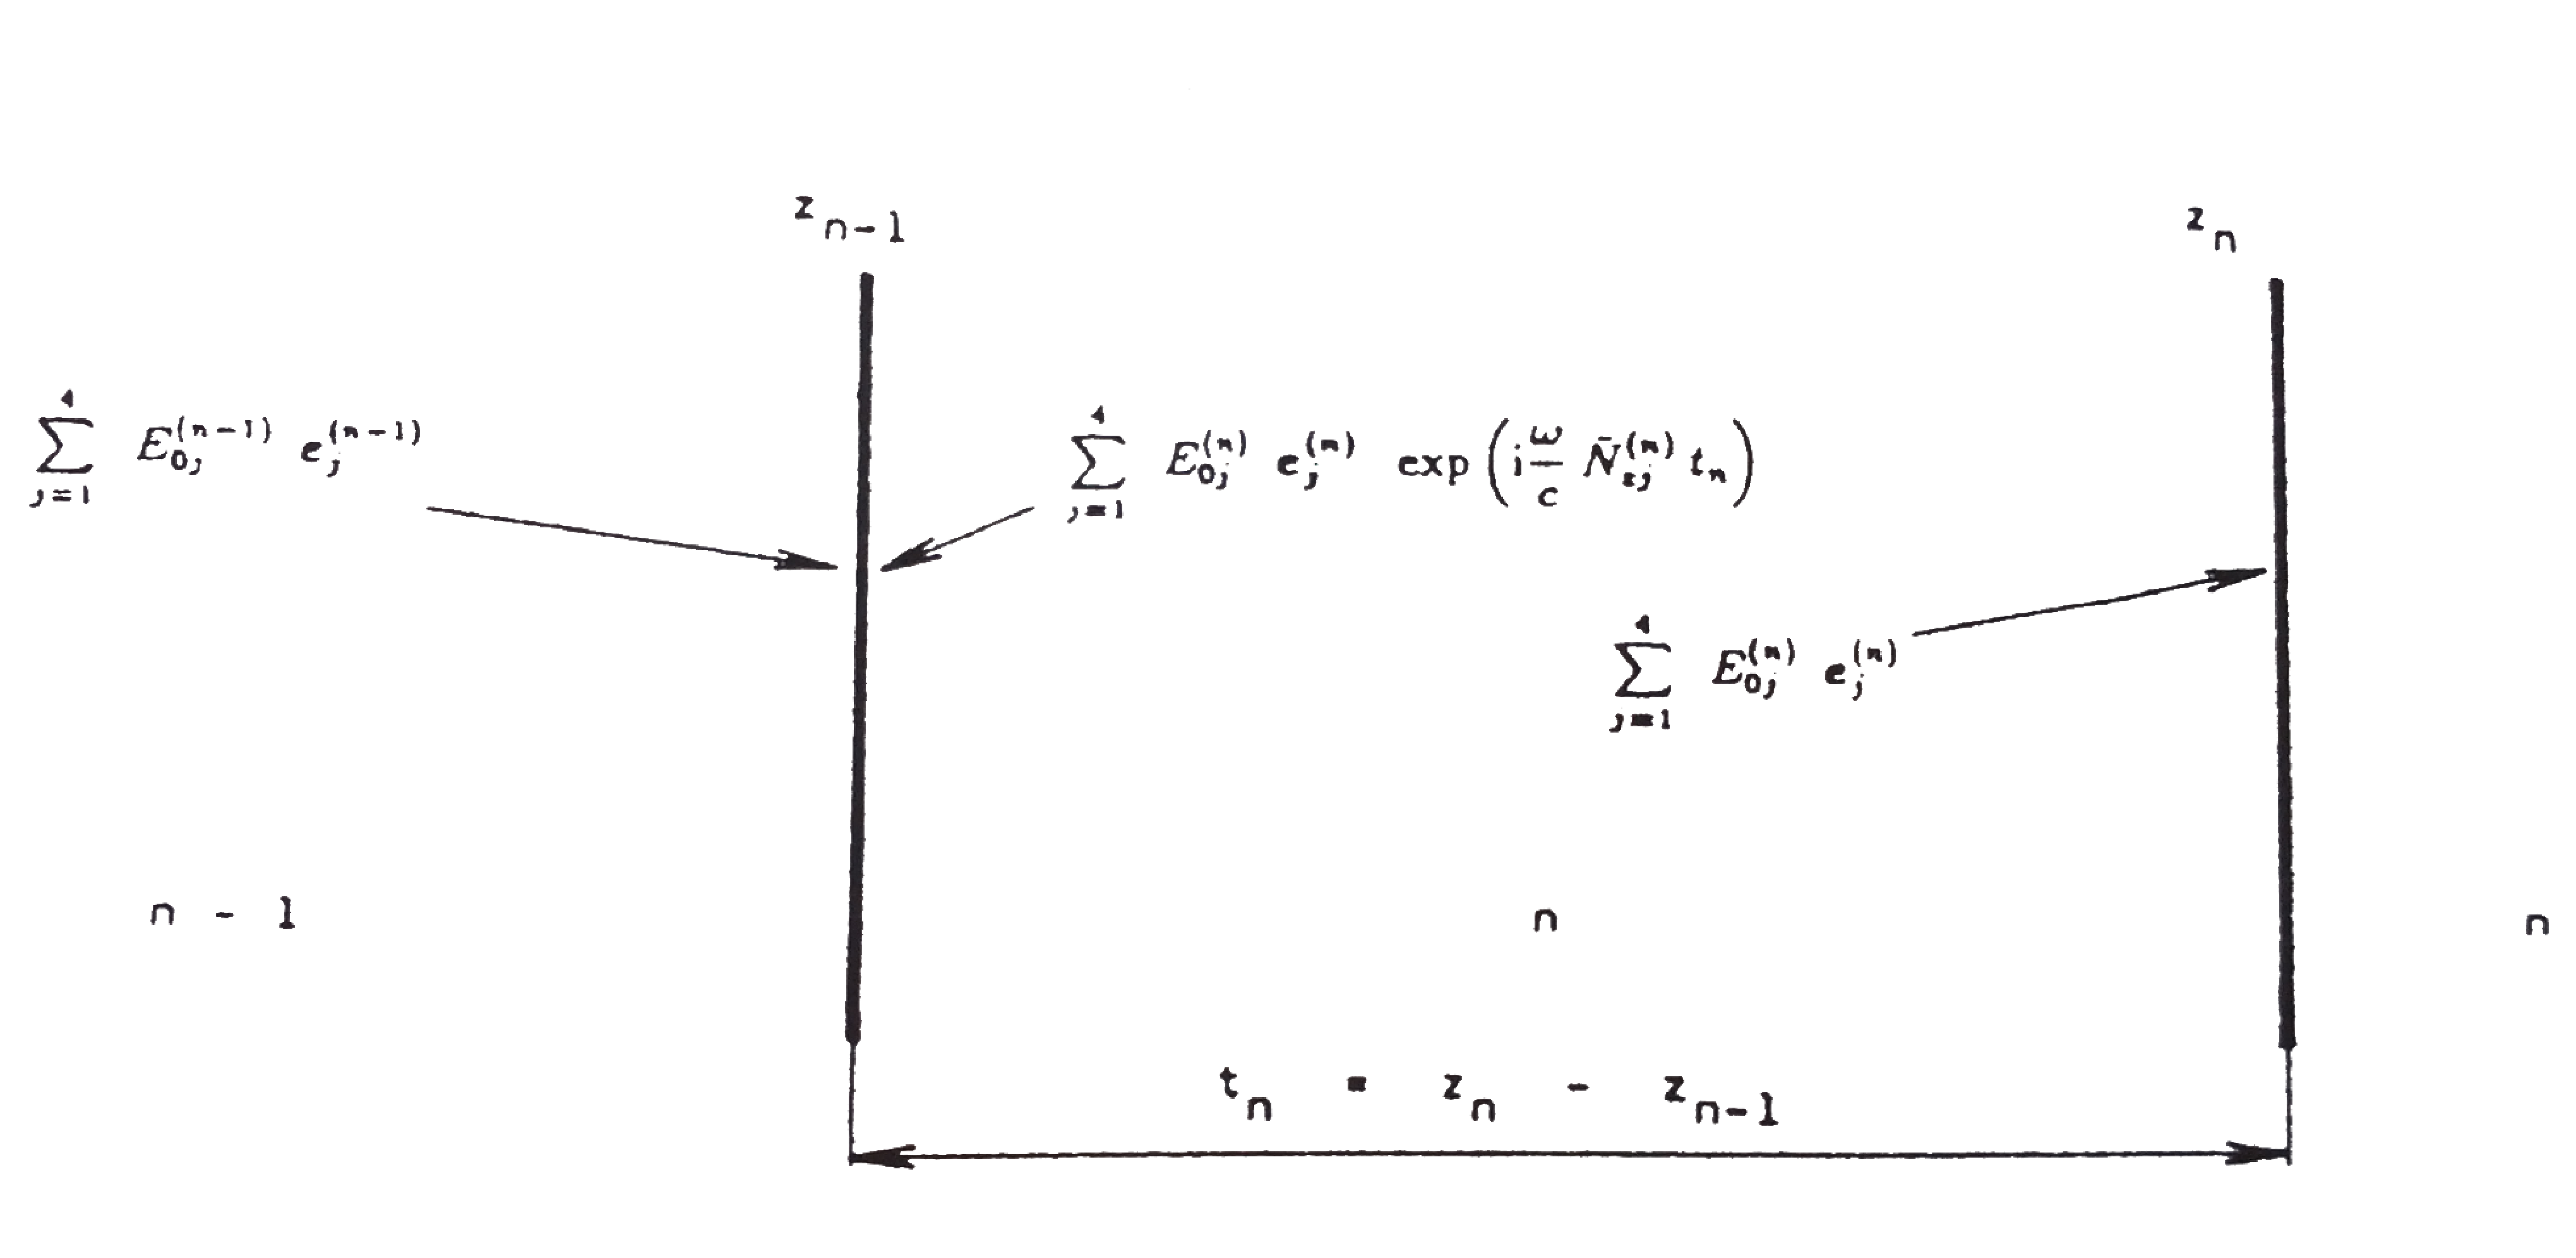
\includegraphics[width=5in]{img/border.eps}
    \end{center}
    \caption{Okrajové podmínky mezi vrstvami}
\end{figure}

Dále bez odvození uvádíme okrajové podmínky na rozhraní n-té a (n-1)-ní vrstvy. Jedná se o soustavu čtyř rovnic pro $E_x$, $E_y$, $B_y$ a $B_x$
\begin{eqnarray}
\sum^4_{j=1}E_{0j}^{(n-1)}(z_{n-1})\vec{e}_j^{(n-1)}\cdot\vec{i}_x &=& \sum^4_{j=1}E_{0j}^{(n)}(z_n)\vec{e}_j^{(n)}\cdot\vec{i}_x \mbox{exp}\left(i\frac{\omega}{c}N_{zj}^{(n)}t_n\right), \\
\sum^4_{j=1}E_{0j}^{(n-1)}(z_{n-1})\vec{b}_j^{(n-1)}\cdot\vec{i}_y &=& \sum^4_{j=1}E_{0j}^{(n)}(z_n)\vec{b}_j^{(n)}\cdot\vec{i}_y \mbox{exp}\left(i\frac{\omega}{c}N_{zj}^{(n)}t_n\right), \\
\sum^4_{j=1}E_{0j}^{(n-1)}(z_{n-1})\vec{e}_j^{(n-1)}\cdot\vec{i}_y &=& \sum^4_{j=1}E_{0j}^{(n)}(z_n)\vec{e}_j^{(n)}\cdot\vec{i}_y \mbox{exp}\left(i\frac{\omega}{c}N_{zj}^{(n)}t_n\right), \\
\sum^4_{j=1}E_{0j}^{(n-1)}(z_{n-1})\vec{b}_j^{(n-1)}\cdot\vec{i}_x &=& \sum^4_{j=1}E_{0j}^{(n)}(z_n)\vec{b}_j^{(n)}\cdot\vec{i}_x \mbox{exp}\left(i\frac{\omega}{c}N_{zj}^{(n)}t_n\right).
\end{eqnarray}
Tato soustava popisuje lineární transformaci amplitud příslušných módů. Velmi výhodné je její přepsání do maticové rovnice
\begin{eqnarray}
\mathbb{D}^{(n-1)}\vec{E}_0^{(n-1)}(z_{n-1})=\mathbb{D}^{(n)}\mathbb{P}^{(n)}\vec{E}^{(n)}_0(z_n),
\end{eqnarray}
kde čtvrtá komponenta vektoru $\vec{E_0^{(n)}}$ je koeficient $E^{(n)}_{0j}(z_n)$. Prvky propagační matice $\mathbb{P}$ jsou dány
\begin{eqnarray}
\mathbb{P}_{ij}^{(n)}=\delta_{ij} \mbox{exp}\left(i\frac{\omega}{c}N_{zj}^{(n)}t_n\right).
\end{eqnarray}
Řádky dynamické matice $\mathbb{D}$ jsou pak dány komponentami příslušných polarizací
\begin{eqnarray}
\mathbb{D}_{1j}^{(n)}=\vec{e}_j^{(n)}\cdot\vec{i}_x, \\
\mathbb{D}_{2j}^{(n)}=\vec{b}_j^{(n)}\cdot\vec{i}_y, \\
\mathbb{D}_{3j}^{(n)}=\vec{e}_j^{(n)}\cdot\vec{i}_y, \\
\mathbb{D}_{4j}^{(n)}=\vec{b}_j^{(n)}\cdot\vec{i}_x.
\end{eqnarray}
Abychom se nemuseli zabývat obencným řešením těchto rovnic, využijeme toho, že při polární magnetizaci má tenzor permitivity tvar (\ref{epsilon polar}). To vede na zjednodušené rovnice
\begin{eqnarray}
\mathbb{D}_{1j}^{(n)}&=& -\varepsilon_{xy}(\varepsilon_{xx}-N_y^2)+\varepsilon_{xx}N_yN_z, \\
\mathbb{D}_{2j}^{(n)}&=&N_{zj}[-\varepsilon_{xy}^{(n)}(\varepsilon_{zz}^{(n)}-N_y^2)], \\
\mathbb{D}_{3j}^{(n)}&=&(\varepsilon_{zz}^{(n)}-N^2_y(\varepsilon_{xx}^{(n)}-N_y^2-(N_{zj}^{(n)})^2), \\
\mathbb{D}_{4j}^{(n)}&=&-(\varepsilon_{xx}^{(n)}-N_y^2-N_{zj}^{(n)2})N_{zj}^{(n)}\varepsilon_{zz}^{(n)})
\end{eqnarray}
díky kterým sjme schopni určit celou dynamickou matici.
Pro $m$ vrstev pak získáme výsledný vztah pouhým násobením matic
\begin{eqnarray}
\begin{split}
\vec{E}_0^{(0)}(z_0) = [\mathbb{D}^{(0)}]^{-1}\mathbb{D}^{(1)}\mathbb{P}^{(1)}[\mathbb{D}^{(1)}]^{-1}\dots \mathbb{D}^{(m)}\mathbb{P}^{(m)}[\mathbb{D}^{(m)}]^{-1}\mathbb{D}^{(m+1)}\vec{E}_0^{(m+1)}(z_m)\\
=\mathbb{M}\vec{E}_0^{(m+1)}(z_m)
\end{split}
\end{eqnarray}
Z matice $\mathbb{M}$ můžeme následně vypočítat reflexní a trasmisní koeficienty, jako poměr apmlitudy dopadajícího a odraženého, či prošlého pole, s uvážením, že z $E^{(n)}$ nic nedopadá. Ve zkratce získáme vztahy %TODO ověřit
\begin{eqnarray}
r_{12}=\frac{\mathbb{M}_{21}\mathbb{M}_{33} - \mathbb{M}_{23}\mathbb{M}_{31}}{\mathbb{M}_{11}\mathbb{M}_{33}-\mathbb{M}_{13}\mathbb{M}_{31}}, \\
r_{14}=\frac{\mathbb{M}_{41}\mathbb{M}_{33}-\mathbb{M}_{43}\mathbb{M}_{31}}{\mathbb{M}_{11}\mathbb{M}_{33}-\mathbb{M}_{13}\mathbb{M}_{31}}, \\
r_{31}=\frac{\mathbb{M}_{11}\mathbb{M}_{43}-\mathbb{M}_{41}\mathbb{M}_{13}}{\mathbb{M}_{11}\mathbb{M}_{33}-\mathbb{M}_{13}\mathbb{M}_{31}}, \\
r_{32}=\frac{\mathbb{M}_{11}\mathbb{M}_{23}-\mathbb{M}_{21}\mathbb{M}_{13}}{\mathbb{M}_{11}\mathbb{M}_{33}-\mathbb{M}_{13}\mathbb{M}_{31}}.
\end{eqnarray}
Přičemž platí vztah vázající tyto koeficienty s Jonesovou reflexní maticí
\begin{eqnarray}
\begin{bmatrix}
r_{ss} & r_{sp} \\ r_{ps} & r_{pp} 
\end{bmatrix}
= 
\begin{bmatrix} 
r_{12} &r_{32} \\ -r_{14} & -r_{34} 
\end{bmatrix}
\end{eqnarray}
Analogické vztahy platí i pro transmisní koeficienty. Z obou pak můžeme dopočítat příslušné Kerrovy či Faradayovy koeficienty.

\section{Jednoduchá vrstva}
Pokud máme pouze jednu vrstvu na substrátu, můžeme se vyhnout řešení maticové rovnice a použít výraz
\begin{eqnarray}
\Theta_K=\theta_K-i\epsilon_K=\frac{i\varepsilon_2(1-r^2_{01})\left[(1+r^2_{12}e^{-2i\beta_1})(1-e^{-2i\beta_1})+4i\beta_1e^{-2i\beta_1}\right]}{4\varepsilon_1(1+r_{01}+r_{12}e^{-2i\beta_1})},
\label{teor kerr}
\end{eqnarray}
kde $\beta_1=n_1\frac{\omega}{c}t_1=\sqrt{\varepsilon_1}\frac{E}{\hbar c}t_1$ a $r_{01}$ resp. $r_{12}$ jsou Fresnelovy reflexní koeficienty na prvním resp. druhém rozhraní. Pro kolmý dopad pro ně platí
\begin{eqnarray}
r_{ij}=\frac{\sqrt{\varepsilon_j}-\sqrt{\varepsilon_i}}{\sqrt{\varepsilon_j}+\sqrt{\varepsilon_i}}.
\end{eqnarray}
